\documentclass[phd]{byuprop}
% Options for this class include the following (* indicates default):
%
%   10pt -- 10 point font size
%   11pt -- 11 point font size
%   12pt (*) -- 12 point font size
%
%   ms -- produce a thesis proposal (off)
%   areaexam -- produce a research area overview (off)
%   phd -- produce a dissertation proposal (off)
%
%   singlespacing -- single-spaced lines
%   doublespacing -- double-spaced lines
%
%   layout -- show layout lines on the pages, helps with overfull boxes (off)
%   grid -- show a half-inch grid on every page, helps with printing (off)


% This command fixes my particular printer, which starts 0.03 inches too low,
% shifting the whole page down by that amount.  This shifts the document
% content up so that it comes out right when printed.
%
% Discovering this sort of behavior is best done by specifying the ``grid''
% option in the class parameters above.  It prints a 1/2 inch grid on every
% page.  You can then use a ruler to determine exactly what the printer is
% doing.
%
% Uncomment to shift content up (accounting for printer problems)
%\setlength{\voffset}{-.03in}

% Here we set things up for invisible hyperlinks in the document.  This makes
% the electronic version clickable without changing the way that the document
% prints.  It's useful, but optional.  Note that if you use latex instead of
% pdflatex, you should change "pdftex" to "ps2pdf".
\usepackage[
    pdftex,
    bookmarks=true,
    breaklinks=true,
    raiselinks=true,
    pdfborder={0 0 0},
    colorlinks=false,
    ]{hyperref}
    
\usepackage{caption}
\usepackage{subcaption}
\usepackage{bm}
\usepackage{amsfonts}
\usepackage{amsmath}
\usepackage{comment}

\usepackage{amsthm}
\usepackage{multirow}
\usepackage{pbox}

\newtheorem{mylem}{Lemma}
\newtheorem{myhyp}{Assumption}
\newtheorem{myprop}{Property}
\newtheorem{mythm}{Theorem}
\newtheorem{mydef}{Definition}

% Rewrite the itemize, description, and enumerate environments to have more
% reasonable spacing:
\newcommand{\ItemSep}{\itemsep 0pt}
\let\oldenum=\enumerate
\renewcommand{\enumerate}{\oldenum \ItemSep}
\let\olditem=\itemize
\renewcommand{\itemize}{\olditem \ItemSep}
\let\olddesc=\description
\renewcommand{\description}{\olddesc \ItemSep}

% Get a little less fussy about word spacing on a line.  Sometimes produces
% ugly results, so keep your eyes peeled.
\sloppy

% Important settings for the byuprop class. %
%%%%%%%%%%%%%%%%%%%%%%%%%%%%%%%%%%%%%%%%%%%%%

% Because I use these things in more than one place, I created new commands for
% them.  I did not use \providecommand because I absolutely want LaTeX to error
% out if these already exist.
\newcommand{\Title}{
From qualitative to quantitative: Supporting robot understanding in human-interactive path planning
}
\newcommand{\Author}{Daqing Yi}
\newcommand{\SubmissionMonth}{July}
\newcommand{\SubmissionYear}{2015}

% Take these from the commands defined above
\title{\Title}
\author{\Author}
\monthsubmitted{\SubmissionMonth}
\yearsubmitted{\SubmissionYear}

% Committee members
\committeechair{Michael~A.~Goodrich}
\committeemembera{Kevin~D.~Seppi}
\committeememberb{Randal~W.~Beard}
\committeememberc{Mark~J.~Clement}
\committeememberd{Parris~K.~Egbert}

% Department graduate coordinator
\graduatecoordinator{Quinn~Snell}

\documentabstract{%
% The proposal abstract should be 1 to 2 paragraphs.
%This document is an example of how to use the byuprop {\LaTeX} class file.  The class creates Ph.D. and Master's documents equally well, producing all appropriate preamble content and adhering precisely to the minimum formatting requirements.

%Note that there is a blank line between paragraphs, here.
Improvements in robot autonomy are changing human-robot interaction from low-level manipulation to high-level task-based collaboration.
When a robot can independently and autonomously execute tasks, a human in a human-robot team acts as a collaborator or task supervisor instead of a tele-operator.
In planning paths for a robot's motion, it is very important that the supervisor's qualitative intent is translated into a quantitative model so that the robot can produce a desirable consequence.

We propose a series of robot motion-planning algorithms, each of which is designed to support some aspect of a human's intent.
We consider planning problems: planning with a human-motion constraint, planning with a topological requirement, planning with multiple objectives, and modeling them from verbal instructions.
These algorithms create a set of robot affordance that support complex task definition and flexible decision-making.
}

%%%%%%%%%%%%%%%%%%%%%%%%%%%%%%%%%%%%%%%%%%%%%

% Set up the internal PDF information so that it becomes part of the document
% metadata.  The pdfinfo command will display this. Be sure to set the document
% type and add your own keywords.
\hypersetup{%
    pdftitle=\Title,%
    pdfauthor=\Author,%
    %pdfsubject={Document Type, BYU CS Department: %
    %            Submitted \SubmissionMonth~\SubmissionYear, Created \today},%
    pdfsubject={PhD Proposal, BYU CS Department: %
                Submitted \SubmissionMonth~\SubmissionYear, Created \today},%
    pdfkeywords={Multi-Objective Optimization, Homotopy class, Path Planning, Human-Robot Collaboration, Particle Swarm Optimization},%
}

% These packages allow the bibliography to be sorted alphabetically and allow references to more than one paper to be sorted and compressed (i.e. instead of [5,2,4,6] you get [2,4-6])
\usepackage[numbers,sort&compress]{natbib}
\usepackage{hyperref}

% Additional packages required for your specific thesis go here. I've left some I use as examples.
\usepackage{graphicx}
\usepackage{pdfsync}

\begin{document}

% Produce the preamble
\maketitle

%%%%%%%%%%%%%%%%%%%%%%%%%%%%%%%%%%%%%%%%%%%%%%%%%%%%%%%%%%%%%%%%%%%%%%%%%%%%%%%
\section{Introduction}
\label{sec:intro}
% 1-2 pages
% Answers:
% 1) What problem do you want to solve?
% 2) Who cares about this problem and why?

\subsection{Robotic Path Planning in Human-Robot Collaboration}
\label{sec:intro:robotic_path_planning_in_human_robot_collaboration}

The ways robots and humans ``think'' are very different.
Humans are experts at making qualitative decisions, from low-level movement to high-level reasoning,
and robots show great strength in solving quantitative problems like high-speed data processing, high-precision repeated motion, etc.
Robots can
\begin{itemize}
\item deliver constant and stable performance without fatigue;
\item collect versatile formats of observation data by different sensors;
\item access some particular spaces that humans cannot reach; and
\item do repetitive tasks and detailed computations without error, etc.
\end{itemize}
Humans can
\begin{itemize}
\item adapt to environment change in task execution;
\item respond to unexpected occurrences that happen accidentally; and
\item be robust to vague or conflicting pieces of information. 
\end{itemize}
In organizing humans and robots in a team, the differences between humans and robots cannot be ignored.
Due to the differences, humans and robots are often assigned different roles when collaborating in a team.
In teamwide collaboration, there is often a team task, which is defined as the goal of the team.
A team ``coach'' splits the team task into subtasks for team players.
In the spirit of human-centered intelligence, we assume that the team ``coach'' is a human who executes high-level planning, splits tasks, and schedules teammates.
The team players include both humans and robots.
%In general, human's strengths include high-level decision-making and robot's strengths include low-level operations.  
For example, in a search-and-rescue task, robots perform dull, dirty and dangerous tasks, and alert a human only when an abnormality is detected~\cite{Nourbakhsh2005}.
The human then deals with abnormal occurrences.
The robot players explore regions that are inaccessible and dangerous to the humans, and assist the human players when needed.
Particularly when situations change, the human players are needed to organize the robot players to react.

Because task requirements from a human coach are usually qualitative~\cite{brenner2007mediating}, how they can be precisely interpreted by robots into quantitative optimization problems is a big challenge.
When a few requirements are ambiguous or difficult to describe, an interactive processes can be used to identify the human intent.
Moreover, we have to consider the collaboration between the human players and the robot players in task execution.
For example, there might exist constraints between the human's motion and the robot's motion in evaluating the team performance~\cite{Yi2014a}.
Generally, the robot is expected to translate qualitative information from the human into quantitative path planning.

\subsection{Translating qualitative information into quantitative path planning}
\label{sec:intro:modeling_qualitative_information_into_quantitative_path_planning}

Allowing a human to use qualitative instructions to guide a robot simplifies the human's task.
%Expressing qualitatively simplifies humans instructing robots, which is essential to the prevalence of human-robot interaction. 
In modeling a path-planning problem, qualitative information needs to be translated into quantitative information, including geographic information, objectives to be optimized, and constraints.
From the qualitative perspective, we are interested with several phenomena in humans' expression.

\begin{itemize}

\item {\em Humans tend to describe task instructions by natural language.}
Language is an efficient way for humans to communicate, and robots are expected to communicate with humans by language~\cite{Kollar:2010:TUN:1734454.1734553,howard2014natural}. 
There are a few accomplishments in supporting robots to speak.
But how robots can (a) understand verbal instructions from human and (b) translate them into path-planning problems is not yet well answered. 
The robots do not only need to read verbal instructions into qualitative semantic structures, but also to construct quantitative models that can be computed by processors.
%Semantic elements can mean differently in different semantic structures of different sentences.
%The problem creation also depends on the shared spatial common grounds between teammates.
A key problem is establishing a shared spatial common ground between the humans and the robot teammates.

\item {\em There often exist multiple objectives in a human's instructions.}
In planning a path, there is often more than one factor to consider~\cite{Ahmed2013}.
For example, in motion-planning for a rescue task, a human coach might hope a robot's search not only covers the most likely regions but also the risky regions that humans should avoid~\cite{Yi2014}.
Therefore, in modeling path-planning in this domain, there are two objectives: maximizing information and minimizing the risk cost.
If the robot is also expected to reach some goal soon, minimizing the path length should be added as a new objective.
Human preferences on different objectives are often qualitative, which sometimes are difficult to represent by quantitative weights.
Moreover, the objectives can conflict or be incomparable.
Therefore, the robot needs to model multi-objective path planning problems and find solutions by prior or posterior information~\cite{Miettinen1999} that the human coach gives.

\item {\em Usually humans have topological preferences for some planned paths.}
Spatial constraints, such as those created by finding a path through obstacles, divide paths into different topologies~\cite{Bhattachary2010}.
It is natural that a human coach has preference for some path topologies~\cite{Yi2014}.
These preference may come from task requirements, team scheduling constraints, or the properties of an agent.
These topological differences can be represented by either a soft path shape constraint or a preference ranking.
For example, the human coach hopes that a robot goes to some goal location as quickly as possible.
In this case, there is no hard constraint of visiting some regions while avoiding some other regions.
But visiting several regions, which means the paths belong to specific homotopic classes, is implicitly helpful to the performance, i.e. safety.
This type of qualitative information can be important to the task performance and should not be ignored in planning paths.

\end{itemize} 

In the remain of this proposal, we will propose our requirements and claims using the above phenomena in human-robot interaction for path-planning problems.
Then we will propose algorithms to support the proposed requirements and the claims.

%%%%%%%%%%%%%%%%%%%%%%%%%%%%%%%%%%%%%%%%%%%%%%%%%%%%%%%%%%%%%%%%%%%%%%%%%%%%%%%
\section{Related Work}
\label{sec:related_work}

In this section, we review the research studies in mental models in robot motion planning.
Then we discuss related work with specific topics that we are interested in.

%%%%%%%%%%%%%%%%%%%%%%%%%%%%%%%%%%%%%%%%%%%%%%%%%%%%%%%%%%%%%%%%%%%%%%%%%%%%%%%
%\subsection{Research Area Overview}
\subsection{Mental Models in Path Planning}
\label{sec:related_work:mental_models_in_path_planning}
% Research Area Overview
% Describes the broad research area (citing the 20 most important papers)
% Should be about 3 pages and may be in the Introduction or Related Work
% sections or may be an appendix.

In the literature on human-machine interaction, mental models play key roles.
Operationally, a mental model is a presentation of how current states are turned into consequences through the actions of an agent~\cite{gray2014manipulating}.
When we have humans and robots in a team, a shared mental model is used as a hypothetical construct that models and explains certain coordinated behaviors of teams.
It provides a framework of mutual awareness, which serves as the means by which an agent selects actions that are consistent and coordinated with those of its teammates~\cite{nikolaidis2012human,Yen_implementingshared,FSS149109,Jonker:2010:SMM:2018118.2018128,Neerincx2011,Mathieu2000,Kennedy2007}.
Figure \ref{fig:team_info_flow} illustrates the information flow in the shared mental model of the coach-based human-robot team described above.

A human's intent can be operationally defined as a preference over consequences produced by a robot's actions and possibly as a preference over the actions used by the robot to produce a desirable consequence.
Because a robot's task is given by a human coach in a human-robot team, information flows from the human coach's mental model to the team players' mental models.
Correctly modeling the human's intent determines the performance of task execution.
However, the humans' intents are often qualitative descriptions, which are difficult to be translated into quantitative models that the robots operate on.

\begin{figure}[hbtp]
\centering
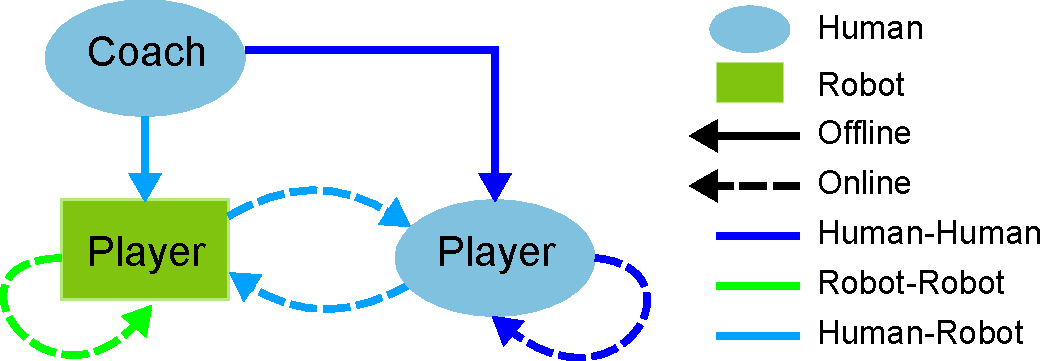
\includegraphics[width=0.6\linewidth]{./fig/team_info_flow.pdf}
\caption{The information flow in the team.}
\label{fig:team_info_flow}
\end{figure}

In path-planning problems, the mental model provides goals and preferences for evaluating the performance of tasks.
These goals and preferences are used to find the optimal paths for task execution~\cite{choset2005principles}.
Current research work focus on introducing new features to the robotic mental models for creating new affordances, especially in interpreting humans' mental models.
In human-machine interaction, affordance refers to the perceived and actual properties of the thing, primarily those fundamental properties that determine just how the thing could possibly be used, see, for example, in~\cite{norman2013design}.
Planning for a task consists of two steps:
\begin{enumerate}
\item modeling a task into an optimization problem; and
\item solving the optimization problem to get path solutions.
\end{enumerate}

We are proposing work that explore how to translate a human's qualitative intents into problems with quantitative models, and how to solve the problems.
A qualitative map description is one common type of qualitative information associated with a human's mental model~\cite{kuipers1999}.
Based on a human-sketched map, a probabilistic topological structure can be created to model a map with uncertainty~\cite{Shah2013}.
Observations in navigation are used to correct the probabilistic topological structure, which is used as an estimated map.
Planned paths are then adjusted online by the changes in the estimated maps.
Qualitative information can also be represented by geometrical relations~\cite{mcclelland2012qualitative,mcclelland2014qualitative} with landmarks.
Within the constraints of feasibility, the estimated map structure can be updated by noisy sensory measurements.

Another important type of qualitative source is human language~\cite{tellex2011understanding,walter2014framework}.
Natural language instructions can be used as observations in the robotic SLAM problem.
Three layers of maps, which are semantic, topological and metric, are maintained in a graphical model structure~\cite{walter2014framework} so that the input can be either noisy sensor measurement or fuzzy verbal description.
Both sensor information and human's online instructions can be merged into an environmental learning process~\cite{6301744,5509521,ahmed2014enabling}.
By using the Bayesian filter framework, human information is loaded into a softmax likelihood model so that it can be merged into Bayesian update.
%New affordances in human-robot interaction are created by extending the ways of communication in mental models and supporting more features of problem definitions.

%%%%%%%%%%%%%%%%%%%%%%%%%%%%%%%%%%%%%%%%%%%%%%%%%%%%%%%%%%%%%%%%%%%%%%%%%%%%%%%
%\subsection{Research-Related Work}
\subsection{Algorithm-Specific Work} 
\label{sec:related_work:algorithm_specific_work}
% Related Work
% 1-2 pages
% Answers:
% 3) What have others done to solve this problem and why is this inadequate?
%    (only a small overlap with the area exam from the introduction)

In order to support the phenomena we mentioned in Section \ref{sec:intro:modeling_qualitative_information_into_quantitative_path_planning}, we now review several fields that are related.
In how to model problems, we review some literature in modeling problems from verbal instructions.
In how to support problem solving, we review studies in path-planning problems with submodularity, homotopy and multiple objectives.

\subsubsection{Model Problems from Verbal Instructions}
\label{sec:related_work:algorithm_specific_work:model_problems_from_verbal_instructions}

Current human-robot communication relies heavily on training human operators, which means that the operators need customize information for robots.
This prevents human-robot interaction being applied in more fields.
The goal of the proposed research is supporting a robot in modeling problems based on natural information of human.

In planning paths, spatial information in the language is a very important source to a mental model.
A spatial semantic hierarchy is usually maintained in the mental model, which represents the information relationship from the sensory to the topological and the metrical~\cite{kuipers1999}.
There have been a few grammars introduced to parse sentences into semantic elements by task specifications, e.g. SDC (Spatial Description Clause)~\cite{tellex2011understanding} and TBS (Tactical Behavior Specification)~\cite{Boularias_2015_7953}.
Grounding the semantic elements with meanings behind is an understanding process~\cite{Kollar:2010:TUN:1734454.1734553}.
In path planning, problems are often framed as optimization problems that seek to find paths best match semantic meanings~\cite{tellex2011understanding,Boularias_2015_7953}.
This approach can be strengthened by integrating multiple information sources, such as visual sensors and odometers~\cite{6696569}.

Planners have been proposed to infer a human's intent from a human's verbal instruction~\cite{howard2014natural,Duvallet2014}.
In such planners, groundings are extracted from semantics in a working environment.
The verbal instruction is parsed into phrases by the grammar of the Spatial Descriptive Clause. 
A factor graph is then created to model correspondences between groundings and phrases.
Some labeled training dataset can be used to train the factor graph model.
After training, the factor graph model can be used to infer the groundings of verbal instructions.

\subsubsection{Multiple Objectives in Path Planning}
\label{sec:related_work:algorithm_specific_work:multiple_objectives_in_path_planning}

Tasks assigned to robots are complex which means that they can be performed in several different ways.
This complexity leads to the requirement that the robot must make tradeoffs among several different objectives.
For example, a robot in a search task may be expected to maximize the coverage area while minimizing energy consumption and avoiding risk; see, for example~\cite{Mei2005,Yi2014}. 
As another example, a robot manipulator may need to satisfy performance criteria related to movement, joint velocities, joint accelerations, etc.~\cite{Pires2004}.

A common method of finding a solution of a multi-objective optimization problem is optimizing the single objective created by a weighted sum of the multiple objectives.  
In path-planning with multiple objectives, the properties of the path produced by this method are determined by how the objectives are weighted. 
This means that a programmer, designer, or human teammate must decide how to assign the weights so that the quantitative behavior matches the intent.  
In addition to the burden placed on the human operator, optimizing a weighted sum does not work when the multiple objectives are very difficult to compare or are expressed in incommensurate units.

In solving a multi-objective optimization problem, the output is often a set of non-dominated solutions, which are also often called Pareto-optimal solutions~\cite{Miettinen1999}.
``Non-dominated''  means that each solution is at least better in one objective or equally the same in all the objectives when compared with any other solution.
In this proposed work, we assume that there can be an interactive process where a human selects one solution from the set of Pareto-optimal solution~\cite{Marler2004}.
In multi-objective path-planning, a set of Pareto-optimal paths could be found as well.
The Pareto-optimal path that best matches the human's intent can be selected as the solution that best balances tradeoffs between the objectives.

Most popular methods in multi-objective optimization are not naturally applicable to path-planning~\cite{Zhang2007,Deb2014}.
One approach to addressing this issue is to change the representation for a path by coding a path as a sequence of fixed-length line segments represented by directions~\cite{Ahmed2013,Howlett2006} or waypoints~\cite{Sujit2009,Pires2004} so that an evolutionary algorithm can be applied. 
Unfortunately, these approaches do not scale well for large problems, and estimating the required number of segments is very challenging. 
Another approach is to represent the path as a point in a very high-dimensional vector space.
In this approach a path is represented as a point in a $ n * d $ dimensional space formed by $ n $ different  $d$-dimensional way-points~\cite{Ahmed2011,Ahmed2013}.
However the search can be very difficult if we allow the number of way-points and, therefore, the dimensionality of the optimization problem to vary. 
The algorithm does not work well when the obstacles in the path-planning space introduce discontinuities in these high-dimensional spaces, which limits the applicability of heuristic-based search approaches~\cite{Sujit2009,Zhang2007}.
There is still the need of an algorithm that can efficiently and effectively find a set of Pareto-optimal paths for a given set of objectives.

\subsubsection{Homotopy in Path Planning}
\label{sec:related_work:algorithm_specific_work:homotopy_in_path_planning}


Unlike a point solution in common optimization problems, a path is not only evaluated by its fitness/cost but also its shape.
Humans often represent the world using a topological-based rather than metric-based path planning~\cite{Aginsky1997,kuipers1999}. 
Various methods have been used to create topological-representations that can be used by path-planners for robots~\cite{Mataric1992,Thrun1998,Fasola2013,Shah2013}.
Obstacles in a map divide paths into topological groups by the similarities in the shapes of the paths. 
The topological notion of {\em homotopy} presents a formal definition of the similarity between two paths. 
This definition can be used both to determine the similarity between two paths as well as to partition paths into different classes.

Homotopy-based path planning requires an algorithm to determine the homotopic equivalence of two paths, which is usually computationally expensive. 
There are a few research studies that focus on effectively and efficiently identifying the homotopy class to which a path belongs or determining the homotopic equivalence of two paths. 
The Voronoi diagram is used to identify a path from any homotopy class in~\cite{Banerjee2013}. 
By converting any path into a simple path from the Voronoi diagram, the homotopy class of the path can be determined. 
However there exist limitations on finding some paths in a map with complex obstacles in this approach.
By applying the funnel algorithm in the universal covering space, the minimum-length path is efficiently optimized in a given homotopy class in~\cite{Hershberger1994}. 
Similar to the Voronoi approach, the complexity of the problem is increased when the shapes of the obstacles are not smooth and convex. 
Semi-algebraic cuts are used to convert paths into “words” so that the homotopic equivalence can be recognized into~\cite{Grigoriev1998}. 
Also, the Cauchy Integral theorem has been introduced to determine the homotopic equivalence of any two paths by marking some positions in obstacles as undefined~\cite{Bhattachary2010}. 
Given two paths sharing the same start and goal, we can determine whether there is an obstacle inside a region that is enclosed by two paths by the value of the complex integral. 
Because the map is discretized, the computation cost expands greatly if some complex obstacles are reasonably approximated by the cells.
How to efficiently and effectively find the optimal paths in different homotopy classes is still an open question.

\subsubsection{Submodularity in Path Planing}
\label{sec:related_work:algorithm_specific_work:submodularity_in_path_planning}

Search is a very important task in path planning.
In planning motion for a search task, the objective is usually to maximize the information collected with a limited motion resource.
Because an observation at a time covers a region around the search agent, using a coverage model for the robot makes the path planning a {\em maximum coverage problem}.
Maximum coverage is known to be a classic NP-hard combinatorial optimization problem~\cite{Megiddo1983} because coverage overlap cannot be ignored. 
Mutual information is introduced to measure the total information
of a set of observation coverages, which implies a property of
“nondecreasing submodularity”~\cite{Singh2009}. 
A greedy approximation with a known performance bound can efficiently exploit the submodularity property of mutual information~\cite{Singh2009}. 
A branch and bound approach can also be used in informative path
planning~\cite{Binney2012}.

Maximizing the reward collected from a limited-length graph walk is usually known as an orienteering problem~\cite{Vansteenwegen2011}, in which the total reward is a sum of the rewards of visited vertices. 
If the reward function of a vertex has the submodularity property as in a maximum coverage problem, the problem is defined as a submodular orienteering problem~\cite{Chekuri2005}. 
Unfortunately, in the submodular orienteering case the location of the robot at time $ t $ constrains the reachable locations at time $ t+1 $.
Thus, naively applying a greedy algorithm to the submodular orienteering case, that is, with a “teleport” assumption, yields poor results~\cite{Krause2012}. 
For a generalization of the submodular orienteering problem in which the neighboring constraint can be converted into time budget, a recursive greedy algorithm can be applied~\cite{Chekuri2005}.
If the planning is considered for a human-robot team as we are proposing, the collaboration and the constraints between team players cannot be ingored.
When we import the constraints from a human teammate's behavior to the submodular path planning, this solution won't work any more. 


%%%%%%%%%%%%%%%%%%%%%%%%%%%%%%%%%%%%%%%%%%%%%%%%%%%%%%%%%%%%%%%%%%%%%%%%%%%%%%%
\section{Thesis Statement}
\label{sec:thesis_statement}
% 1 to 2 sentences

In robotic path planning, algorithms can transform a human's qualitative requirement into a robot's quantitative model so that the robot behavior satisfies the human's intent.
In particular, algorithms can be created that allow a human to express multi-objective and topological preference, and can be built to use verbal communication.

%%%%%%%%%%%%%%%%%%%%%%%%%%%%%%%%%%%%%%%%%%%%%%%%%%%%%%%%%%%%%%%%%%%%%%%%%%%%%%%
\section{Project Description}
\label{sec:project_description}
% about 6-8 pages
% Answers:
% 4) What is your proposed solution to this problem?

We will model the following aspects of information flow from a human to a robot: 
\begin{itemize}
	\item How to support multiple objectives in tasks,
	\item How to support human's topological preference, and
	\item How to model problems from a language instruction.
\end{itemize}
After they have been modeled into path-planning problems, we will propose algorithms to solve the problems and provide analyses and simulations to support the algorithms.
Table \ref{tb:requirement} shows how the list of model requirements abobe can be interpreted as a general type of problem from the literature, and identifies an algorithm that we propose to solve the problem for path-planning in a human-robot team.

\begin{table}
\begin{center}
{\renewcommand{\arraystretch}{3}
\begin{tabular}{|l|l|l|l|}
	\hline
	\multicolumn{2}{|l|}{ \textbf{Requirement} } & \textbf{Problem} & \textbf{Algorithm} \\ \hline
	\multicolumn{2}{|l|}{ \pbox{20cm}{Support multiple objectives in \\ tasks} }  & Multi-objective path planning & MORFF $^{*}$ \\ \hline
	\multicolumn{2}{|l|}{\multirow{2}{*}{ \pbox{20cm}{Support humans' topological\\ preference} }}  & \pbox{20cm}{Submodular path planning with \\ reference path constraint} & Wingman path planning \\ \cline{3-4} 
	\multicolumn{2}{|l|}{ }  & Homotopy-based path planning  & HA-RRT$^{*}$ \\ \hline
	\multicolumn{2}{|l|}{ \pbox{20cm}{Model problems from verbal\\ instructions} } & \pbox{20cm}{Grounding multiple objectives and \\ topological preference in \\ natural language} & \pbox{20cm}{ CDCG \\ HDCG } \\ \hline
\end{tabular}
}
\end{center}
\caption{Project description.}
\label{tb:requirement}
\end{table}

\subsection{Multi-Objective Path Planning}
\label{sec:project_description:multi_objective_path_planning}

To support a complex decision with multiple objectives, we define a multi-objective path planning and propose an algorithm to find solutions.

When there are multiple objectives in a task, the goal is to find a solution that trades off between the objectives.
%When there exists conflicts between the objectives, the goal is then finding a solution that is a good trade-off between the objectives.
A common method for finding a solution of a multi-objective optimization problem is to optimize a single objective created by a weighted sum of the multiple objectives.
This means that either a programmer, designer , or a human teammate must decide how to assign the weights so that the qualitative behavior matches what is intended. 
Optimizing a weighted sum does not work when the multiple objectives are very difficult to compare or are expressed in incommensurate units.
Thus, it will be better if a set of Pareto-optimal paths is firstly found and the human teammate can select one from them.

Given this context, we now define the multi-objective path-planning problem to find a set of Pareto-optimal paths.
Consider a multi-objective path-planning problem defined on a bounded, connected open set $X\subset\mathbb{R}^d$ of possible solutions, and $K$ different objectives $\{c_{1}(\cdot), c_{2}(\cdot), ... c_{K}(\cdot)\}$. 
Without loss of generality, assume that each $c_{k}(\cdot)$ is a cost function such that the objective is to minimize these functions.  
Since the Pareto-optimal set of paths in $ \mathbb{R}^{d} $ is not enumerable, the {\em goal is to find a representative, finite ($M$-element) subset of the Pareto-optimal set}.  
By ``representative" we mean a diverse set of solutions that span the Pareto set rather than, for example, several points clustered in a single region of the Pareto set.

In contrast to searching through and comparing solutions in order to find a Pareto-optimal set, we use a decomposition-based method similar to MOEA-D~\cite{Zhang2007}.  
MOEA-D is an algorithm that decomposes a multi-objective optimization problem into a set of subproblems.  
Each subproblem uses a weighed combination of the objectives to find specific points in the Pareto set or to guide the search for such points.  
%Because we  will use this subproblem idea in our algorithm, it is useful to introduce some notation.
Let $ \bm{\lambda} = [ \lambda_{1} , \cdots , \lambda_{K}  ]^{T} $ be a weighting vector such that $ \sum_{k=1}^{K} \lambda_{k} = 1 $.  
Let $\{c_{1}(\cdot), c_{2}(\cdot), \ldots c_{K}(\cdot)\}$ denote the $K$-element set of objective functions, let $\bm{c}(x) = [c_{1}(x), c_{2}(x), \ldots, c_{K}(x)]^T$, and let $x$ denote a potential solution.  
Finally, let $ \bm{z}^{\rm utop} = [z^{*}_{1}, \cdots , z^{*}_{K}]^{T} $ denote the so-called Utopia reference vector defined by $  z^{*}_{i} = \min_{ X } c_{i} (x) $. 

\begin{figure}
	\centering
	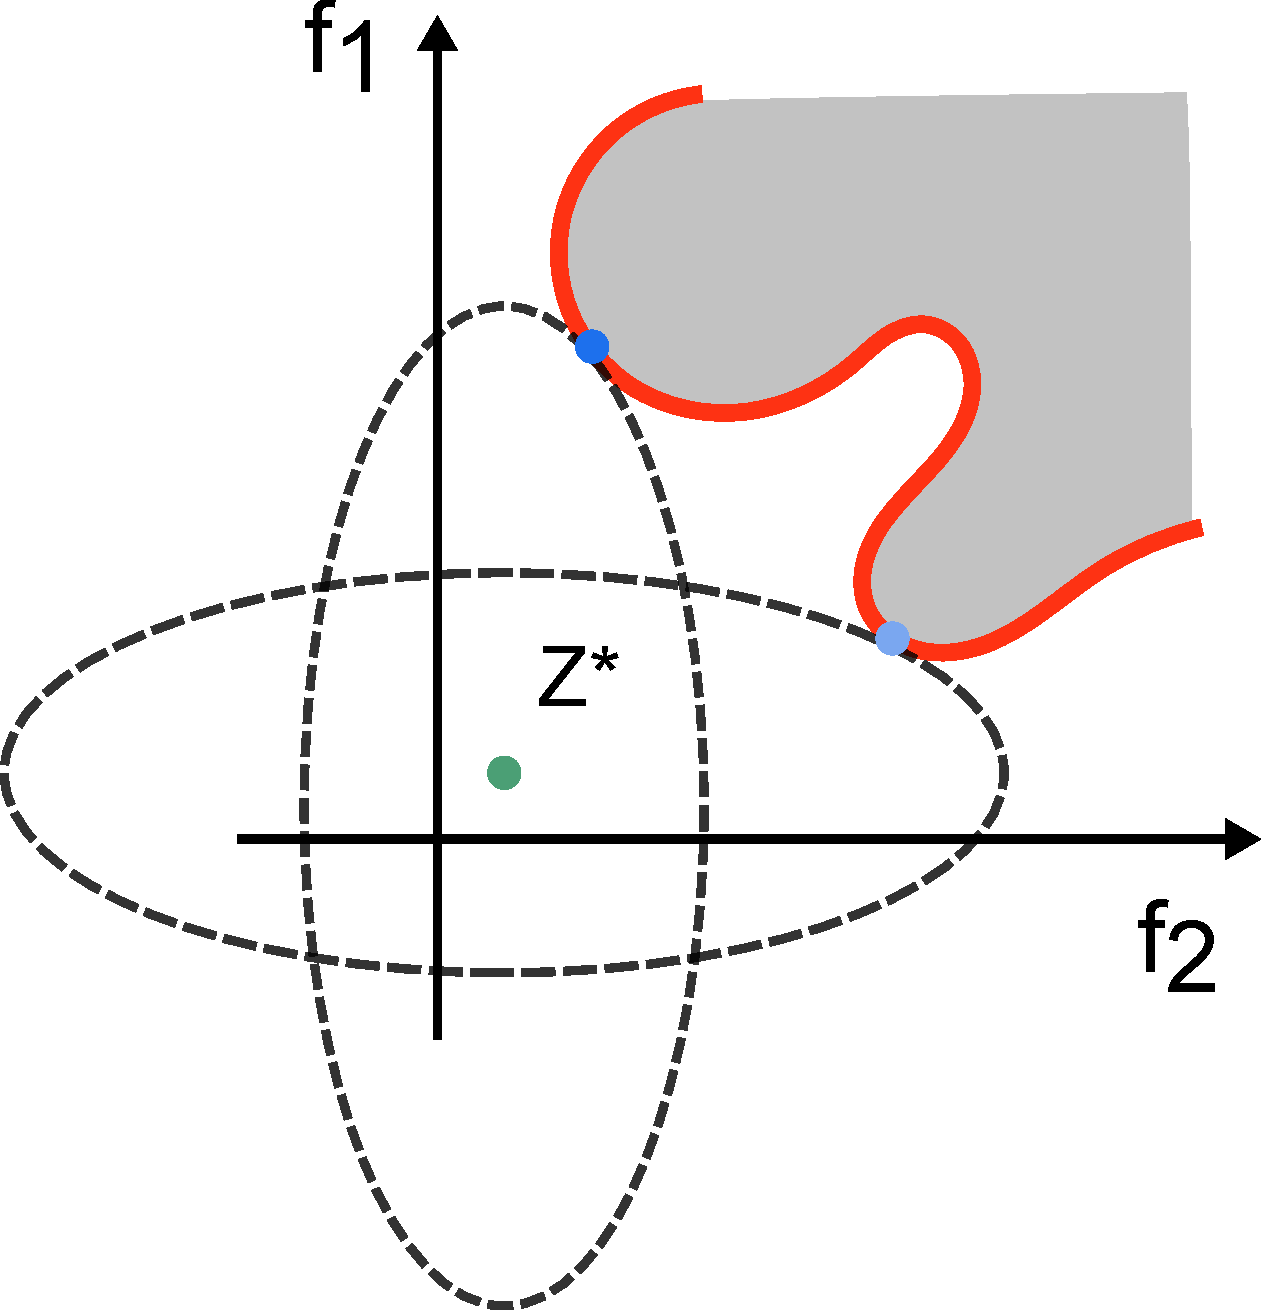
\includegraphics[width=0.3\linewidth]{fig/Tchebycheff}
	\caption{Tchebycheff method of finding Pareto front.}
	\label{fig:Tchebycheff}
\end{figure}

Three types of decomposition methods have been used in prior work~\cite{Zhang2007}.
\begin{eqnarray}
\arg\max_x \sum_{k=1}^{K} \lambda_{k} c_{k} (x) & {\rm Weighted \ Sum} \label{eq:weighted}\\
\arg\min_x\max_{1 \leq k \leq K}  \{ \lambda_{k} | c_{k}(x) - \bm{z}^{\rm utop}_{k}  | \} & {\rm Tchebycheff} \label{eq:Tchebycheff}\\
\arg\min_x \{ d \mid \bm{z}^{\rm utop} - F(x) = d \bm{\lambda} \} & {\rm Boundary \ Intersection \ } \label{eq:boundary}
\end{eqnarray}
The solutions generated by each method are a subset of the Pareto-optimal set.

We propose an algorithm that explores the solution space using RRT$^{*}$-based tree structures but uses multiple trees in the spirit of decomposition-based multi-objective optimization.
Because a set of trees are constructed in the exploration process, we call the algorithm MORRF$^{*}$ (Multi-Objective Rapidly exploring Random Forest$^{*}$).

\begin{figure}
	\centering
	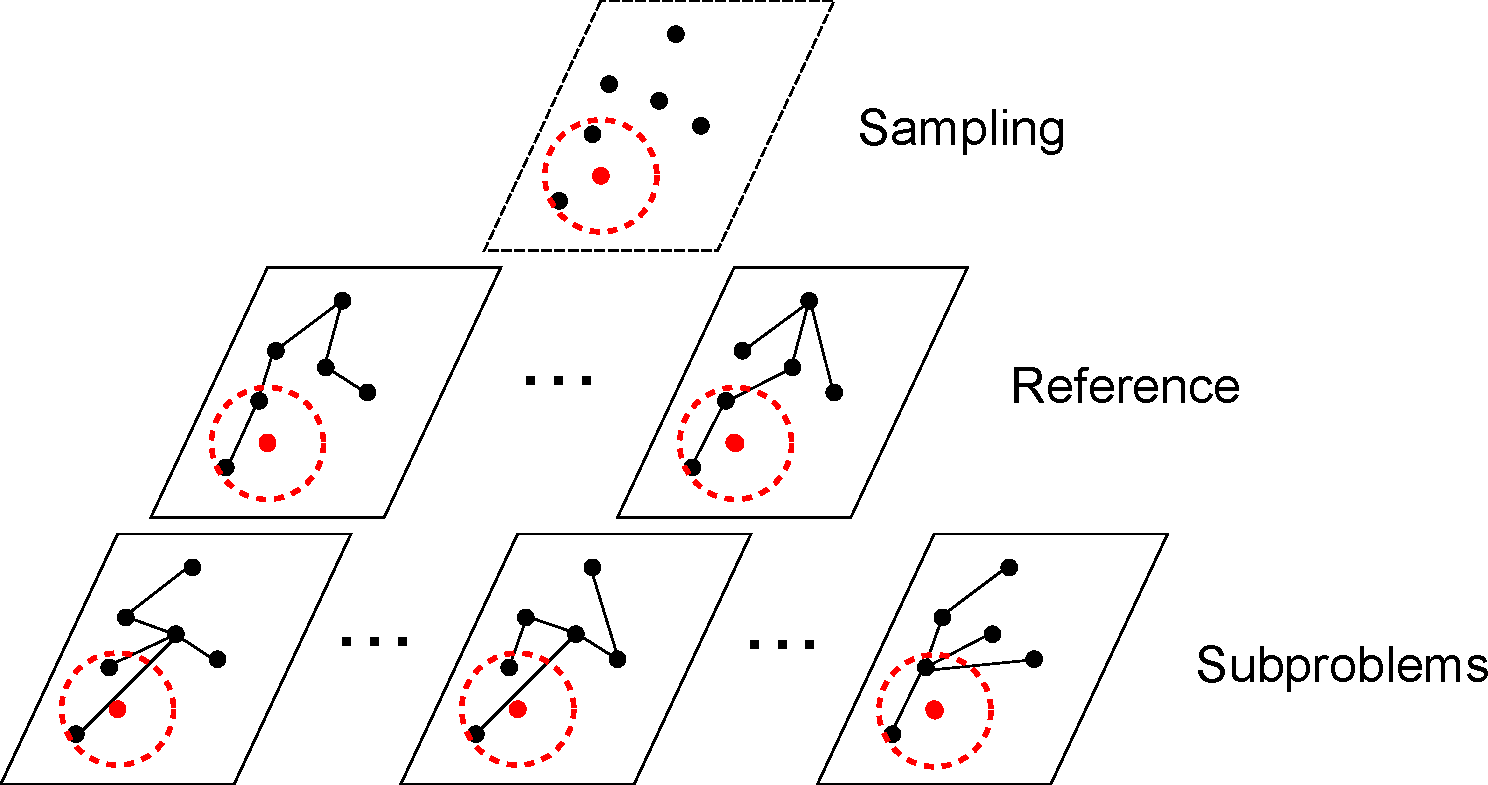
\includegraphics[width=0.55\linewidth]{./fig/MORRTstar}
	\caption{Rapidly exploring process}
	\label{fig:MORRTstar}
\end{figure}

Adopting the idea from the MOEA-D algorithm~\cite{Zhang2007}, the $M$ elements in the solution set $\Sigma^{*}$ will be obtained from $ M $ subproblems decomposed from the multi-objective problem. 
Both the Tchebycheff approach and Boundary Intersection approach require us to define a Utopia reference vector $ \bm{z}^{\rm utop} $ in the fitness space. 
Figure~\ref{fig:Tchebycheff} illustrates how this reference vector is used in a simple (not path planning) two objective problem.  

Take the Tchebycheff approach as an example.
Recall that  $ \bm{\lambda} = [ \lambda_{1} , \cdots , \lambda_{K}  ]^{T} $ is a weighting vector such that $ \sum_{k=1}^{K} \lambda_{k} = 1 $ and that the Tchebycheff approach seeks to find the solution $ x^{te}\in X $ given by $ x^{te} = \arg\min_x \max_{1 \leq k \leq K}  \{ \lambda_{k} | c_{k}(x) - \bm{z}^{\rm utop}_{k}  | \} $.  
As illustrated in Figure~\ref{fig:Tchebycheff}, the Utopia reference vector is defined as the point in cost space that would be obtained if it were possible to find a solution that produced the minimum value for all objectives, that is the $k^{\rm th}$ element of $\bm{z}^{\rm utop}$ is given by $\bm{z}^{\rm utop}_{k} = \arg \min_{x \in X} c_{k}(x)$.  
It is called the ``Utopia'' reference vector because it represents a point that could conceivably be achieved for an ideal point in the solution space.

Given this brief overview of the Tchebycheff method, we now need to extend it to allow for RRT$^{*}$-based sampling of the search space.  
We will need one type of RRT$^{*}$ structure to explore in an attempt to find the Utopia reference vector in cost space and another type of RRT$^{*}$ structure to find paths that minimize the Tchebycheff condition. %, as described below.  
Thus, there are two types of tree structures used for the optimization process.
\begin{itemize}
	\item Each \emph{reference tree} explores using a single objective $ c_{k} (x), k \in K $. 
	The cost of each vertex is calculated by using the $ k^{\rm th} $ objective function.
	\item Each \emph{subproblem tree} explores a subproblem $ g_{m} ( x \mid \lambda_{m} , \bm{z}^{\rm utop} ) , m \in M $.
	The cost associated with each vertex is calculated by using $ g_{m}(x) $ defined by the corresponding approach.
\end{itemize}
Thus $ K $ reference trees are used, one each to explore the minimum of each objective, and $ M $ subproblem trees are used, one for each weighting vector, $ \lambda_{m} $.  
The $K$ reference trees and $M$ subproblem trees constitute the exploration forest.
The solutions obtained from $ M $ subproblem trees constitute a set of Pareto-optimal paths, which are the solutions to the multi-objective path-planning problem. 

\subsection{Involving Topological Preferences in Path-Planning}
\label{sec:project_description:involving_topological_preferences_in_path_planning}

We categorize topological preferences into two types by considering the level of collaboration.
If a human and a robot are constrained in a tight collaborative relationship, the motion of the robot has to be constrained in a region near the position of the human.
A topological preference is defined by a reference path from the human.
By considering the sensor coverage overlap in collaboration, we can model the problem as submodular path-planning problem with a reference-path constraint, which is described in Section~\ref{sec:project_description:submodular_path_planning_with_reference_path_constraint}.
If we ignore the collaboration, the topological preference can then be presented by the homotopy classes in the map.
Therefore, in this case, we can model the problem as homotopy-based path-planning problem in Section~\ref{sec:project_description:homotopy_based_path_planning} 

\subsubsection{Submodular Path-Planning with Reference Path Constraint}
\label{sec:project_description:submodular_path_planning_with_reference_path_constraint}

Before task execution, a coach can assign a subtask for a robot player to explore the world while staying near a human teammate.
For this type of topological preference, the information of the human is given to the robot.
Thus, assuming that the human player's motion can be predicted or is known, the robot player's motion is constrained by the human player's motion, yielding a path-planning problem with a reference-path constraint.
We call this situation in a search task with the {\em robot wingman} problem.

Consider a discretized map of the world formed by a set of cells $ \mathbf{S}$ and suppose that the robot moves with constant speed from any cell to any of its neighbors.
In the search task, each cell in a discretized map is assigned an entropy value, $ H(s) $; to represent the information distribution.
The robot's motion is constrained by a graph topology determined by the cell neighborhood. 
In a period of time of length $ T $, we denote the robot's path as $ X = [x_{1}, x_{2} , \cdots , x_{T}] $.
We adopt an observation coverage model for the robot, which means that the robot can observe not only the cell it currently occupies but also neighboring cells within a given range.
Let the observation at time step $ t $ be $ O^{X}_{t} $, which describes both the observed cells and how well they are observed.
Thus the robot's path $X$, induces a sequence of observations $ \mathbf{O}^{X} = \{ O^{X}_{1}, \cdots , O^{X}_{T-1}, O^{X}_{T} \}$.

We assume that the observation coverage model follows Bayes rule.
Thus we can define the information gain of the robot using mutual information $ I( \mathbf{S} \mid \mathbf{O}^{X} ) =  H( \mathbf{S} ) - H( \mathbf{S}, \mathbf{O}^{X}  ) $.
The entropy reduction over the problem space $ \mathbf{S} $ by the observation $ \mathbf{O}^{X} $ is the {\em information gain} to the robot.

\begin{figure}[hbtp]
\centering
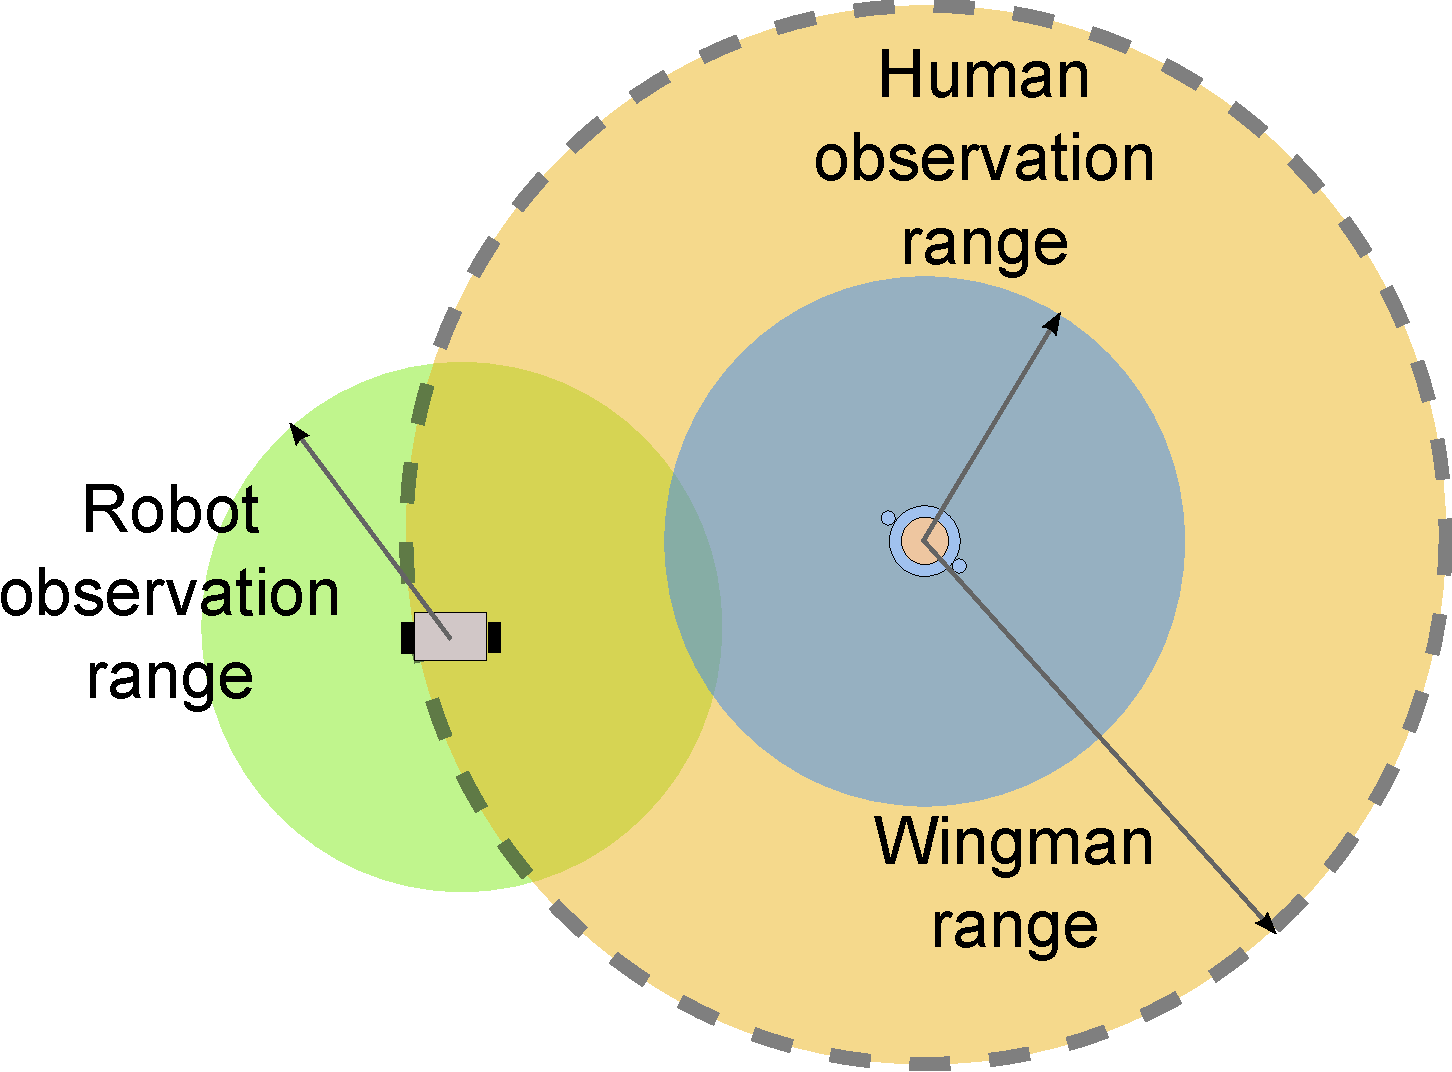
\includegraphics[width=0.37\linewidth]{./fig/Wingman.pdf}
\caption{A Robot Wingman Framework.}
\label{fig:Wingman}
\end{figure}

We select the wingman as a role for the robot player, though there are a few roles that define how the robot's path is constrained by a human.
The wingman role requires that the robot player remains within a tolerance range near around the human player while the human player is moving, as in Figure \ref{fig:Wingman}.
Assume the robot has a model that can predict the human's path.
We denote the human's $T$-step path as $ Y^{h} = [y^{h}_{1}, y^{h}_{2} , \cdots , y^{h}_{T}] $.
We define a neighbor function $ N () $ that represents the assumption that the robot can deviate from a constrained path by no more than a given tolerance.  
At each time step, this neighborhood induces the set of {\em visitable cells} for the robot, which is denoted by $ N( y^{h}_{t} ) $.
Figure \ref{fig:humanConstraint} gives an example.
By organizing the set of visitable cells at time $ t $ into a partition of vertices, we can construct a multi-partite graph $ G = (V, E, T) $ from the constrained path.
A partition $ V(t) \in V $ is obtained from the cells in $ N( y^{h}_{t} ) $.
The edge set $ E $ is determined by the neighborhood of each cell from the discretized map.

Imposing the path constraint $ Y^{h} $, we define the multi-partite graph as follows.
Figure \ref{fig:MultiPartite} illustrates how the path constraint induces the multi-partite graph for a notional human path.
Note that a cell in the discretized map might appear in multiple partitions due to overlaps between sets by $ N( y^{h}_{t} ) $ at different $ t $.

\begin{figure}[htbp]
	\centering
	\begin{subfigure}[t]{0.45\linewidth}
		\centering
		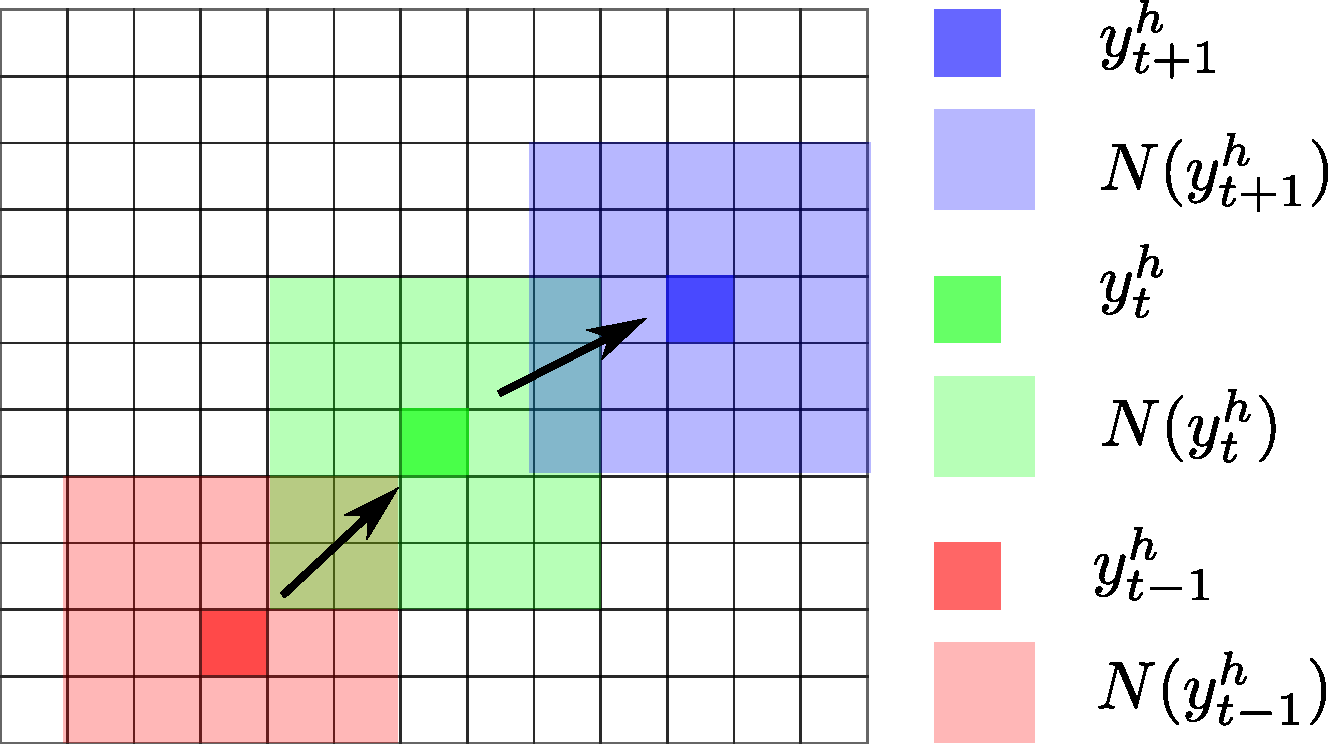
\includegraphics[width=\textwidth]{fig/humanConstraint.pdf}
		\caption{How the multi-partite graph is obtained..}
		\label{fig:humanConstraint}
	\end{subfigure}  
	%\\
	\begin{subfigure}[t]{0.45\linewidth}
		\centering
		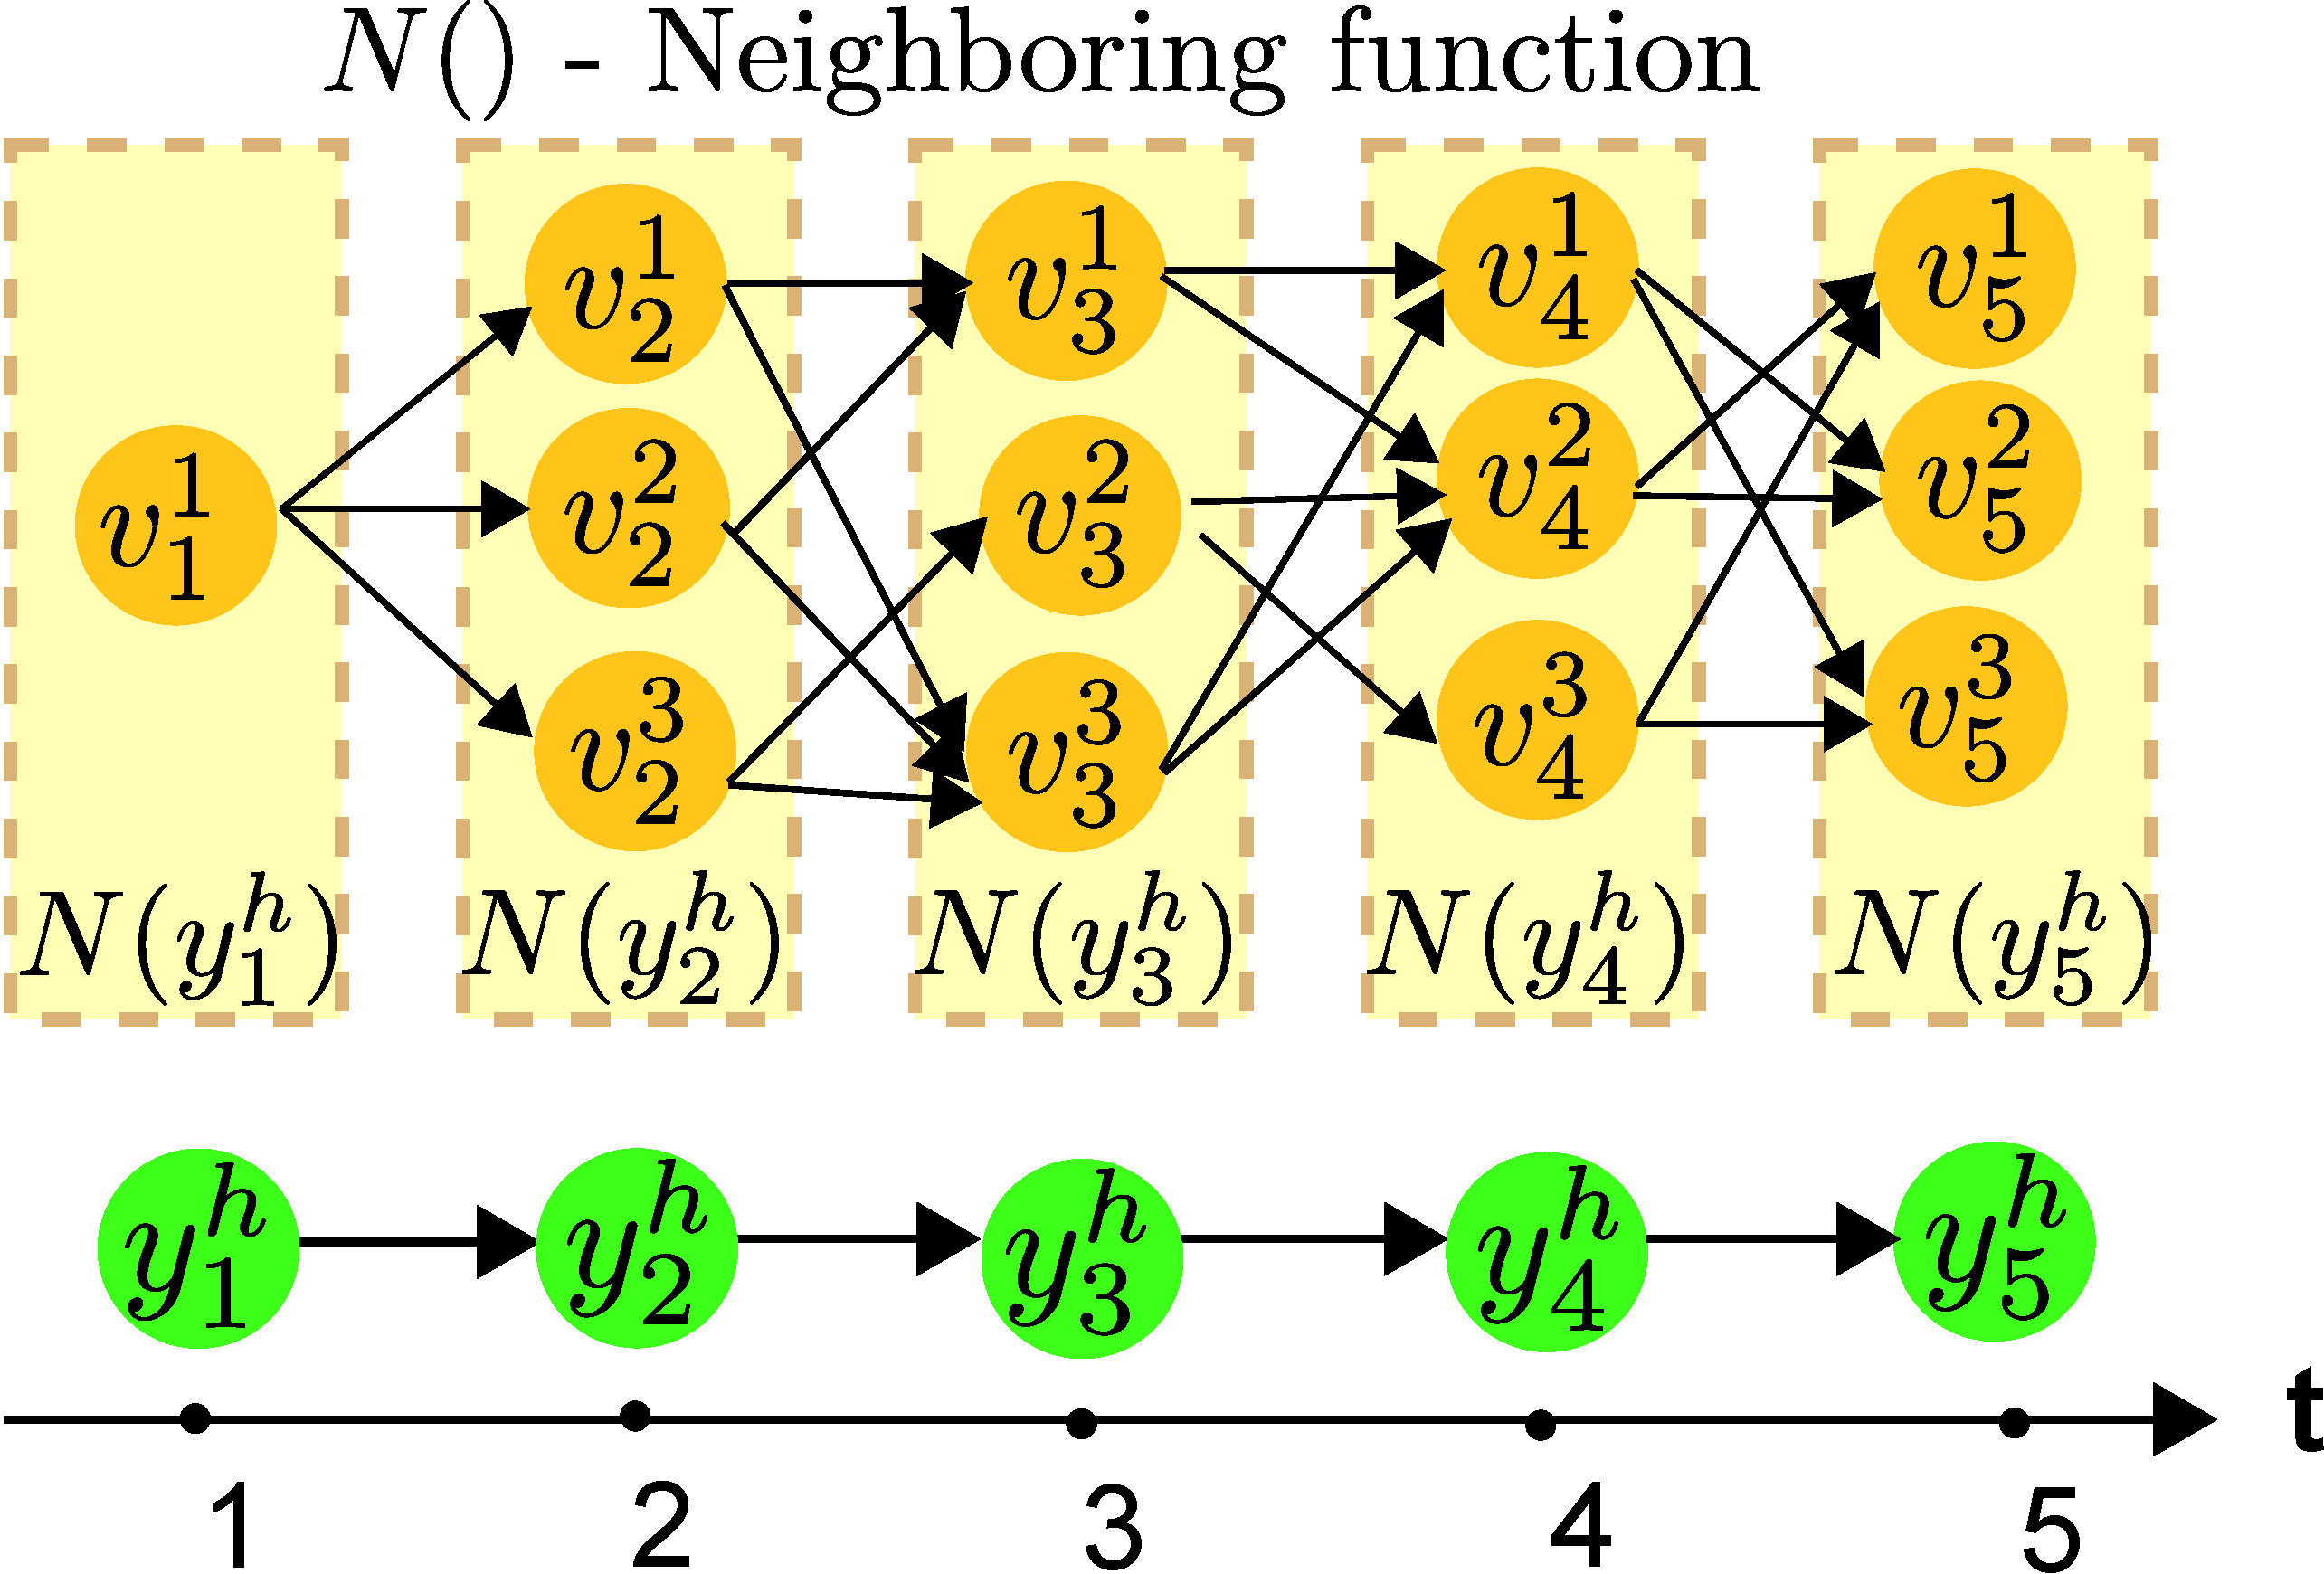
\includegraphics[width=\textwidth]{fig/MultiPartite.pdf}
		\caption{A multi-partite graph from a human path constraint.}
		\label{fig:MultiPartite}
	\end{subfigure}   
	\caption{Reference constraint.}
	\label{fig:reference_constraint}
\end{figure}

In order to guarantee that the search process on a multi-partite graph $ G = (V, E, T) $ always ends with a path of length $ T $, we use a pruning process to ensure that each vertex can be reached from the previous partition and is connected to a vertex in the next partition.
We propose to use backtracking to estimate the maximum total reward and use this estimate as our search heuristic.
We then propose to use an expanding tree to create an anytime algorithm that approximates solution to the submodular orienteering problem on the multi-partite graph.

\subsubsection{Homotopy-based Optimal Path Planning}
\label{sec:project_description:homotopy_based_path_planning}

Observe that, in planning paths for a robot player, a coach may want to express topological constraints like ``go tp the left of the obstacle''.
%some path preference for a subtask is hard for a coach to express.
%The topology of a path is difficult to model into a quantitative model.
The topological concept of \emph{homotopy} is a mathematical formalism of the inherent similarity or dissimilarity of two paths and allows us to precisely quantify such topological constraints.
Given two paths, if one can be deformed into the other without encroaching any obstacle, they are said to be \emph{homotopic}~\cite{Hernandez2015}.
A set of paths that are homotopic to each other forms a \emph{homotopy class}, and the  set of homotopy classes partition the set of all possible paths between any two points $A$ and $B$.
In an environment containing obstacles, the homotopy partition can provide a useful way of grouping paths together based on the similarities of their ``shapes", where the term ``shape'' is interpreted by using the formal topological notion.

In order to support a human intent, expressed as homotopic constraints and preferences, we propose a homotopy-aware RRT$^{*}$ (HA-RRT$^{*}$) algorithm. 
This algorithm uses an RRT$^*$ algorithm to explore possible paths, but each branch of a random tree is aware of the homotopy class to which it belongs. 
We use a set of reference frames for homotopy class identification.

Figure \ref{fig:obs_map:map} shows an example of a map that is decomposed into regions by reference frames (blue and green dash lines).
A \emph{reference frame} is defined as a line segment that connects either two obstacles or an obstacle and a boundary.
A topological graph can be created by the connectivity of decomposed regions.
Each region corresponds to a node in the topological graph.
Each reference frame is adjacent to two regions; thus, it becomes an edge that connects two nodes.
Figure \ref{fig:obs_map:topology} shows a topological graph from the map decomposition in Figure \ref{fig:obs_map:map}.

\begin{figure}[htbp]
	\centering
	\begin{subfigure}[t]{0.27\linewidth}
		\centering
		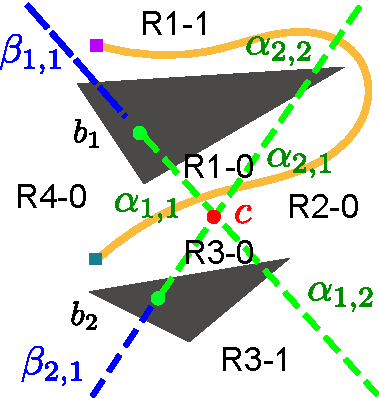
\includegraphics[width=\textwidth]{fig/obs_map.pdf}
		\caption{Decomposition of the map with obstacles.}
		\label{fig:obs_map:map}
	\end{subfigure}  
	%\\
	\begin{subfigure}[t]{0.27\linewidth}
		\centering
		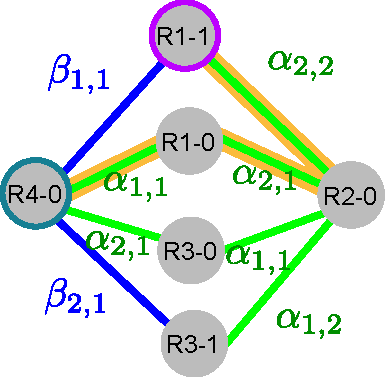
\includegraphics[width=\textwidth]{fig/obs_topology.pdf}
		\caption{The generated topological graph.}
		\label{fig:obs_map:topology}
	\end{subfigure}   
	\caption{Map with obstacles.}
	\label{fig:obs_map}
\end{figure}

Label each reference frame with a \emph{character}.
Each path can be mapped into a {\em string}, which represents the sequence of crossed reference frames.
Following the pattern from \cite{Hernandez2015}, the string can be used to identify the homotopy class of a branch in the RRT.
This means that the growth of a tree can be constrained to a desired homotopy class.
We propose to require each branch of the tree structure tracking a corresponding string as the homotopy information, so that a homotopic constraint can be satisfied and the homotopy classes of all paths can be identified.

We define the set of paths with the same string as a \emph{string class} and use ``$ - $'' to concatenate characters into a string.
Two string classes might still belong to the same homotopy class, e.g, a string class $ \alpha_{1,1}-\alpha_{2,1} $ and a string class $ \alpha_{2,1}-\alpha_{1,1} $ in Figure \ref{fig:obs_map} belong to the same homotopy class.
A homotopic grammar can be used to identify the equivalence.
Also, given one string class, the homotopic grammar can be used to find all the equivalent string classes in the same homotopy class.

With the generated reference frames $ \mathbf{R} $ to identify the homotopy classes, the next question is how to search the optimal paths in the homotopy classes.
RRT$^{*}$ explores the map to generate an optimal tree structure based on the cost distribution in the map.
The homotopy-based path-planning problem essentially looks for the optimal solutions with the constraints of visiting specified regions.
%Because a single optimal tree structure only explores one and only one global best, it cannot support the finding of the optimal solutions in multiple classes.

We propose to use a bidirectional RRT$^{*}$ to obtain the optimal cost-to-come and cost-to-go of different positions.
We can eventually have the optimal path with a via-position constraint by combining (a) the optimal subpath from the start to the via-position with (b) the optimal subpath from the goal to the via-position.
Because the string classes of the branches of both trees are tracked in the exploration process, the optimal path that visits a specific via position can be used to update the optimal paths of the string classes. 
%Thus, in the exploration process, the homotopy class of each branch of the tree is aware.

\subsection{Model Path-Planing Problems from Natural Language Instructions}
\label{sec:project_description:path_planning_with_natural_language_instruction}

A human-natural way of human-robot interaction is to use human language.
%, which is mainly supported by the research in natural language processing(NLP).
Instead of focusing on generic natural language processing problems, we only look at how path-planning problems can be modeled from semantic structures.
The semantic structures are generated from verbal instructions by existing grammar parsers~\cite{Kollar:2010:TUN:1734454.1734553}.
We need to provide methods to infer the task definition from the semantic structures, focusing on the requirements with multiple objectives and topological preferences.

The Tactical Behavior Specification (TBS) language has been introduced as a grammar to support instructions with spatial relations~\cite{Boularias_2015_7953}.
We propose to extend this grammar so that it can be applied in our context.
We propose to extend it in two ways: by grounding adverbs and allowing topological preferences~\cite{Yi2014}.
For example, if a human coach tells a robot that ``go around building A quickly and carefully and then between the two trees while avoiding region C'',
it implies that there potentially exist two objectives from the adverbs, ``quickly'' and ``carefully''.
Practically, this might mean to minimize the path length and minimize the risk.
It also indicates the topology of the path that the human wants: ``around building A'', ``between the two trees'' and ``avoiding region C''.
The semantic structures can be grounded into multi-objective path planning, homotopy-based path-planning or submodular path planning with constraints.
We are going to use a graphical model to infer the relations between the semantics and the groundings.

The graphical model has been a popular tool to model ambiguous relationships between utterances and semantics.
After training by language samples, the graphical model could infer the meaning of verbal language.
Similarly, we can use it to understand a human's verbal commands to a robot.
In the application of path-planning, the human's verbal command is associated with spatial elements. 
Therefore, the Spatial Descriptive Clause(SDC) has been introduced to parse the verbal command into a sequence of phrases~\cite{Kollar:2010:TUN:1734454.1734553}.

The process of assigning physical meanings to phrases is called {\em grounding}.
A verbal sentence is decomposed into phrases $ \lambda^{r}_{i} $, which carry the information from the human.
Grounding variables $ \gamma^{r}_{j} $ are extracted from the map, which include
\begin{itemize}
\item {\em verb fields} : the change in orientation between the viewpoints from verb/action semantic,
\item {\em figure and landmark fields} : the viewpoint transition and the detected objects, and
\item {\em spatial relations} : the functions of the geometries of the paths and the landmarks.
\end{itemize}
By assuming that the groundings are conditionally independent, a conditional random field (CRF) can be used as an undirected graphical model for the relationship between the phrases and the groundings.
Correspondences $ \phi^{k} $ are introduced to indicate whether a grounding element is linked with a phrase from the SDC~\cite{tellex2011understanding},
indirectly, it measures how the grounding variables match the verbal sentence.
Figure \ref{fig:graph_model:induction} gives two examples of how graphical models are created from the SDC.
The corresponding node $ \phi^{k} $ connects the grounding node $ \gamma^{r}_{j} $ and the phrase node $ \lambda^{r}_{i} $.
A labeled dataset can be used to train the graphical model.
The objective of the training is maximizing the likelihood of the correspondences.
\begin{equation}
\arg \max_{\phi_{i,j} \in \Phi } \prod p( \phi_{i,j} \mid \gamma^{r}_{j} , \lambda^{r}_{i} )
\end{equation}
The trained graphical model can then be used to infer the most likely grounding nodes from a given verbal command.

\begin{figure}[htbp]
	\centering
	\begin{subfigure}[t]{0.45\linewidth}
		\centering
		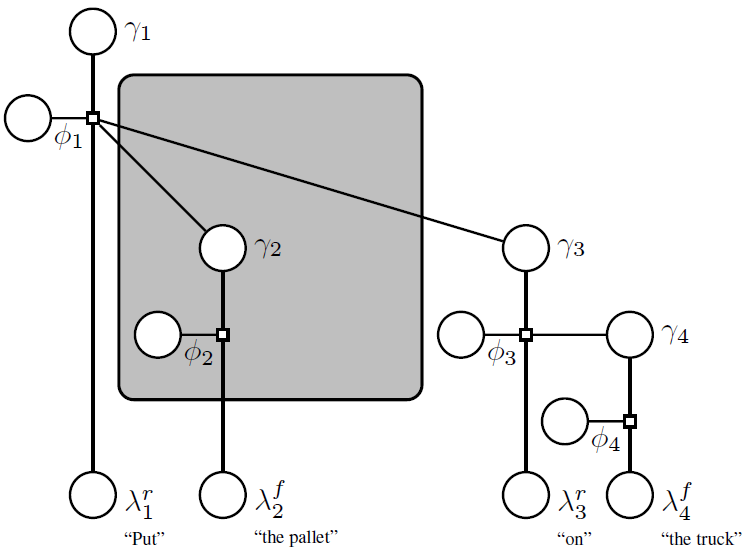
\includegraphics[width=\textwidth]{fig/Induction1}
		\caption{``Put the pallet on the truck.''}
		\label{fig:graph_model:induction1}
	\end{subfigure}  
	%\\
	\begin{subfigure}[t]{0.45\linewidth}
		\centering
		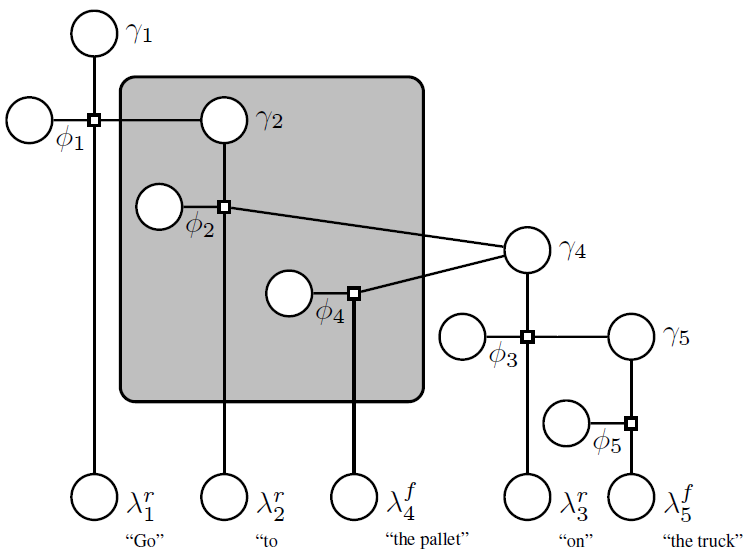
\includegraphics[width=\textwidth]{fig/Induction2}
		\caption{``Go to the pallet on the truck.''}
		\label{fig:graph_model:induction2}
	\end{subfigure}   
	\caption{Graph model of two examples~\cite{tellex2011understanding}.}
	\label{fig:graph_model:induction}
\end{figure}

It is noticeable that some adverbs might mean different things in different contexts.
For example, in a sentence of ``put the pallet carefully on the truck'', ``carefully'' requires a smooth motion. 
But in a sentence of ``walk carefully in the crowd'', ``carefully'' means avoiding collisions with someone else.
It can also define multiple objectives as well, e.g. smoothly moving and collision avoiding simultaneously.
A human language understanding process helps identify the human's intent behind an utterance.
We can create a factor graph to model the correspondence between the adverbs and the intended objectives in different sentences and scenarios~\cite{tellex2011understanding}.
After training, it can be used to infer what kind of objectives that the human intended in the verbal command.

Topological preferences can be extracted from human language.
In~\cite{howard2014natural}, the topological preference is inferred from human language and is used as a hard constraint in path planning.
Sometimes, the topological preference can be a soft constraint.
For example, if a human coach says ``better avoiding region C'', he/she prefers avoiding region C but not necessarily.
The topological preference can also be the order of different homotopy classes.
``Going through between A and B is better than between A and C'' implies a homotopy class via the region between A and B is better than a class via the region between A and C.
We propose to construct a factor graph to represent the preference relationship between the groundings and the verbal phrases.
%The {\em correspondence} nodes are replaced with {\em preference} nodes.
%The preference variable is a real value instead of a boolean value.


%%%%%%%%%%%%%%%%%%%%%%%%%%%%%%%%%%%%%%%%%%%%%%%%%%%%%%%%%%%%%%%%%%%%%%%%%%%%%%%
\section{Validation}
\label{sec:validation}
% 1-2 pages
% Answers:
% 5) How can you demonstrate that this is a good solution?

Essentially, the dissertation statement makes two claims:
(1) verbal instructions with specific grammar restriction can be translated into path-planning problem,
and (2) planning problems with  consideration of humans' intents can be solved.
We will validate each claim by theoretical analyses, and by experiments.
Each claim is supported by proposing a corresponding algorithm.
Theoretical analyses and proofs will be used to support the validity and the performance of the algorithms.
Experiments and simulations will be taken to support the performances of the algorithms.
Table \ref{tb:claim} lists the claims from the project description and identifies the validation used for each claim.

\begin{table}[h]
\begin{center}
{\renewcommand{\arraystretch}{3}
\begin{tabular}{|l|l|l|}
\hline
\multicolumn{2}{|l|}{ \textbf{Claim} } & \textbf{Validation} \\ \hline
\multirow{2}{*}{ \pbox{20cm}{Verbal instructions with \\ specific grammar restriction \\ can be translated into \\ path-planning problems. } } & \pbox{20cm}{ The proposed task grammar converts \\ commands into semantic structures. } & \pbox{20cm}{ Empirical study } \\ \cline{2-3} 
                   & \pbox{20cm}{ The proposed graph models converts semantic \\ structures into path-planning problems. } & \pbox{20cm}{ Empirical study } \\ \hline
\multirow{3}{*}{ \pbox{20cm}{Planning problems that \\ considers human intent\\ can be solved.} }  & \pbox{20cm}{ The solutions of the proposed algorithm \\ asymptotically converge to a set of Pareto \\ optimal paths with multiple objectives. } & \pbox{20cm}{ Theoretical study \\ and simulation } \\ \cline{2-3} 
                   & \pbox{20cm}{ The proposed algorithm returns a near-optimal \\ solution at the first iteration and the solution \\ converges to the optimal after enough iterations. } & \pbox{20cm}{ Theoretical study \\ and simulation } \\ \cline{2-3} 
                   & \pbox{20cm}{ The solutions of the proposed algorithm \\ asymptotically converge to optimal paths \\ of given homotopy classes. } & \pbox{20cm}{ Theoretical study \\ and simulation } \\ \hline
\end{tabular}
}
\end{center}
\caption{Claims and validation.}
\label{tb:claim}
\end{table}

\subsection{Multi-Objective Path Planning}
\label{sec:validation:multi_objective_path_planning}

We propose to prove that the solutions found by the proposed MORRF$^{*}$ algorithm can almost surely converge to be Pareto-optimal.
The proof is split into several steps.
First, we prove that the multi-objective path-planning problem can be decomposed into a set of weighted subproblems;
the path from each subproblem tree is a Pareto-optimal path.
Second, we prove that the solutions of the MORRF$^{*}$ almost surely converge to the answers of the weighted subproblems.
There are two converging processes, namely the convergence of the reference trees and the convergence of the subproblem trees.
The convergence of the subproblem trees depends on the convergence of the reference trees.

We then propose a series of simulation studies that provide evidences that the MORRF$^{*}$ produces a representative set of samples that approximates the Pareto set.
Results from the MORRF$^{*}$ are obtained for path-planning problems with two objectives and three objectives, and are compared to a modified version of the NSGA-II multi-objective path-planning algorithm~\cite{Ahmed2013} as well as a variant of the MORRF$^{*}$ that uses a weighted sum approach.
NSGA-II was selected because evidence suggests that it provides more uniform samples from the Pareto set than other approaches~\cite{Deb2002}.

\subsection{Reference Path Constrained Optimal Path Planning}
\label{sec:validation:reference_path_constrained_optimal_path_planning}

We will prove that the solution produced by the wingman algorithm converge to the optimal.
The proof will be split in two steps.
The first step is proving that the backtracking process proposed will never underestimate the maximum reward, by utilizing the submodular property of the problem.
The next step is showing that given enough run time, the proposed algorithm can always find an optimal solution.
This will be proved by showing that a proposed pruning process will never ``freeze'' a node that is in the optimal path.
By using contradiction, we can show that the optimal path can always be found if there is enough run time.

We propose to apply experiments in a world of hexagonal cells,  discretized from a two-dimensional search space.
We will define several metrics to measure the performance of the proposed algorithm.
We will use a \emph{fully expanded tree size} to measure the \emph{problem size}, which depends on the planning length and the vertex connectivities.
Due to the human constraint, the planning length is determined by the human's path length.
The performance of the heuristic is measured by the \emph{percentage of optimal at first iteration}, that is a percentage computed from the value obtain in the first iteration of the proposed algorithm over the optimal value.
We will use the \emph{percentage of nodes explored} to indicate the efficiency of the anytime algorithm framework.
In particular, we are interested in whether freezing nodes improves search efficiency.
In the anytime algorithm, the exploration might not stop when the optimal is found, due to the existence of overestimation.
If the current best solution of a search can reach the optimal very quickly, it means that the best solution found in a fixed time has high probability of being optimal.
We will use the \emph{number of iterations reaching optimal (normalized)} to measure this optimal search capability of the proposed algorithm.

The backtracking heuristic will be compared with the greedy heuristic in experiments to show the advantage in the performance.
We will test the algorithm with different types of workspaces and different types of human reference paths to show the robustness of the algorithm.


\subsection{Homotopy-based Optimal Path Planning}
\label{sec:validation:homotopy_based_optimal_path_planning}

We will provide theoretical proof that the proposed algorithm can find the optimal solutions in a given homotopy classes.
We will show that with the support of a bidirectional tree structure, the solutions of the HA-RRT$^{*}$ gradually converge to the best paths in the given homotopy classes.
The proof requires that both of the trees are from each of the two directions converge to the optimal structures.
Then, given a via-position, the optimal subpath from the start to the via-position and the optimal subpath from the end to the via-position can be found.
The concatenation of the two optimal subpaths makes the optimal path from the start to the goal with the via-position constraint.
As we can identify the string class that each path belongs to, we can restrict the optimal paths to specific string classes.
By a homotopic grammar, we can find the optimal path in each given homotopy class.

We also implement experiments to show how the HA-RRT$^{*}$ can support different types of human intent on the topology.
Consider the following list of ways in which a human can express intent about path shape and corresponding homotopy-based constraints:
\begin{enumerate}
\item \emph{I want the path to visit a sequence of specific regions.}
\item \emph{I want the path to visit some regions and avoid other regions.}
\item \emph{I prefer some path shapes over others, but I recognize that trade-offs may be needed.} 
\item \emph{I have preferences over paths, but I need help in understanding these preferences.}
\end{enumerate}
We will use a demonstration to show that the algorithm enables each type of constraint.

\subsection{Problems Modeled from Verbal Instructions}
\label{sec:validation:understanding_verbal_command}

We will show how verbal instructions can be modeled into optimization problems.
This will be done in two steps.
The first is parsing verbal instructions into semantic structures by a task grammar.
The second is grounding elements in semantic structures into problems, especially multiple objectives and topological preferences.

We will test how the verbal instructions can be parsed into semantic structures by a parser that is defined by a task grammar.
How a semantic structure can be modeled into a path-planning problem is essentially a machine learning problem.
We will prepare training datasets and testing datasets.
We will verify the learning capability of a proposed factor graph structure.
We will propose the measurement method for calibrating how well the human's intent is identified.
Based on the measurement of intent identification, we can collect the successful rate from the statistics.
The performance of the factor graph can be supported by the successful rates of the training datasets and the testing datasets.


%%%%%%%%%%%%%%%%%%%%%%%%%%%%%%%%%%%%%%%%%%%%%%%%%%%%%%%%%%%%%%%%%%%%%%%%%%%%%%%
\section{Dissertation Schedule}
\label{sec:dissertation_schedule}
% about 1/2 page
% specifying dates for completion of major milestones, including potential
% papers and their submission dates

\begin{itemize}
\item Conference Paper: Toward Task-Based Mental Models of Human-Robot Teaming: A Bayesian Approach. (HCII 2013, July 2013)
\item Conference Paper: Supporting Task-oriented Collaboration in Human-Robot Teams using Semantic-based Path Planning. (DSS 2014, June 2014)
\item Conference Paper: Path Planning with a Human
Path Constraint. (IEEE SMC 2014, October 2014)
\item Conference Paper: Input-to-State Stability Analysis on Particle Swarm Optimization. (GECCO 2015, July 2015)
\item Conference Paper: MORRF$^{*}$ : Sampling-based Multi-Objective Motion Planning. (IJCAI 2015, July 2015)
\item Journal Paper: Understanding the Particle Swarm Optimization by component decomposition. (TEVC, Submitted by June 2015)
\item Conference Paper: Homotopy-Aware RRT$^{*}$ : Toward Human-Robot Topological Path-Planning. (AAAI 2016, Submitted by September 2015)
\item Conference Paper: Understanding adverbs in natural language instructions : a
cost-function learning approach (HRI 2016, Submitted by October 2015)
\item Submission of the dissertation to advisor (March 2016)
\item Journal Paper: Sampling-based Multi-Objective Path Planning (Submitted by September 2016)
\item Conference Paper: Robotic environment learning with human instructions (IJCAI 2016, Submitted by February 2016)
\item Submission of the dissertation to committee members (April 2016)
\item Dissertation Defense (June 2016)
\item Journal Paper: Finding the optimal path planning with different homotopy classes (Submitted by April 2016)
\end{itemize}

\appendix

\section{PSO Stability Analysis}
\label{sec:pso_stability_analysis}

Besides the information from a human to an autonomous agent (robot), we also investigate how the information flow between autonomous agents.
We analyze the consensus reaching problem in a team of autonomous agents.
As learned from \cite{1470210}, we introduce input-to-state stability analysis~\cite{Jiang2001} to each agent in the system, which assists the analysis of  consensus reaching.
We apply it to Particle Swarm Optimization problem(PSO).
In PSO, each particle is an independent agent.
Each particle has its own subtask of seeking the optimal.
Random factors are imported for search dynamics.
At the same time, each particle maintains local information (a personal best) and receives neighboring information (a global best).
The consensus reaching is defined that all the particles agree with where the optimal is, so that they share the same global best and personal best.
This is usually called the convergence of the particles.

Although the input-to-state stable analysis can be applied to many versions of PSO,
for this work we use the formulas from Kennedy's most recent definition of PSO~\cite{Bratton2007} for the constricted position-update rule. 
The constricted position-update rule is

\begin{subequations}
\label{eq:pso_alg}
\begin{equation}
\label{eq:up_vel}
\begin{aligned}
v_{ij}(k+1) = \chi [ v_{ij}(k) 
+ \phi^{P} u^{P}_{ij}(k) (x^{P}_{ij}(k) - x_{ij}(k))
 + \phi^{G} u^{G}_{ij}(k) ( x^{G}_{ij}(k) - x_{ij}(k)) ],
\end{aligned}
\end{equation}
\begin{equation}
\label{eq:up_pos}
x_{ij}(k+1) = x_{ij}(k) + v_{ij}(k+1).
\end{equation}
\end{subequations}
$ x_{ij}(k) $ represents the position of particle $ i $ in dimension $ j $ at time $ k $.
Similarly, $ v_{ij}(k) $ represents the velocity of particle $ i $ in dimension $ j $ also at time $ k $.
$ x^{G}_{ij}(k) $ and $ x^{P}_{ij}(k) $ are global best and personal best positions observed by the swarm and the particle respectively. 
$ u^{G}_{ij}(k) $ and $ u^{P}_{ij}(k) $ are independent random values drawn from $ [0,1] $.
$ \chi \in ( 0, 1 ) $, $ \phi^{P} $ and $ \phi^{G} $ are algorithm parameters.

\begin{figure}[htbp]
	\centering
	\begin{subfigure}[t]{0.6\linewidth}
		\centering
		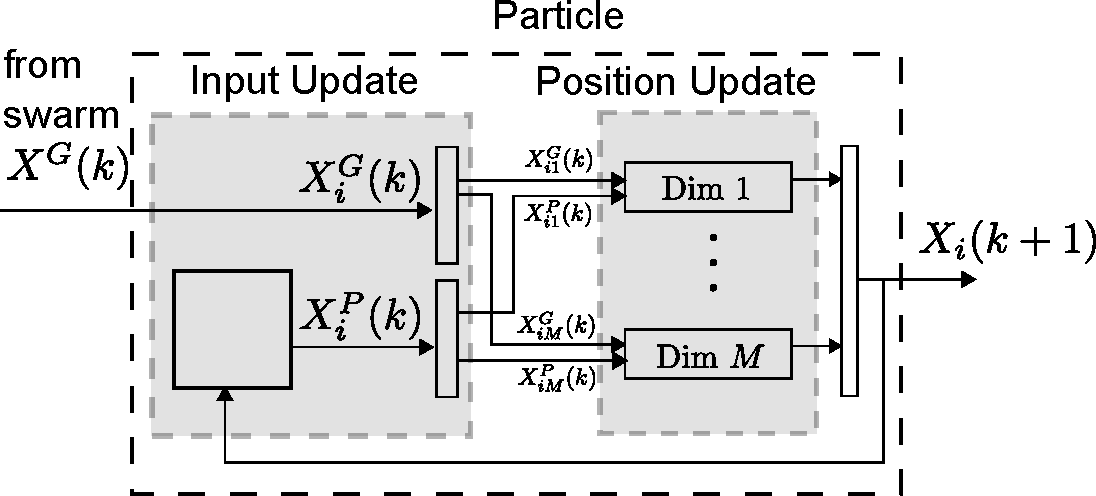
\includegraphics[width=\textwidth]{fig/particle_sys_flow.pdf}
		\caption{System structure of Particle.}
		\label{fig:sys:particle}
	\end{subfigure}  
	%\\
	\begin{subfigure}[t]{0.37\linewidth}
		\centering
		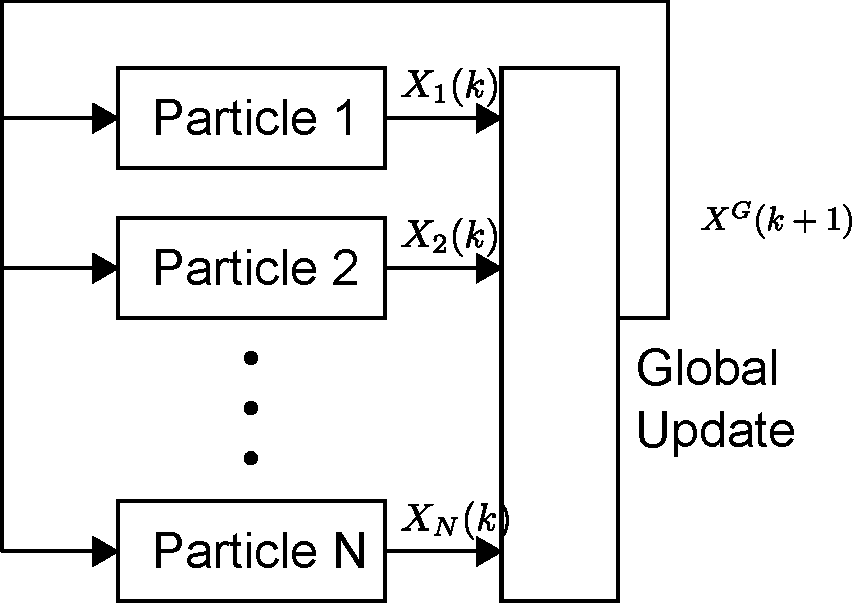
\includegraphics[width=\textwidth]{fig/pso_sys_flow.pdf}
		\caption{System structure of Swarm.}
		\label{fig:sys:swarm}
	\end{subfigure}   
	\caption{System structure of PSO.}
	\label{fig:sys:pso}
\end{figure}

For the input-to-state stability analysis we decompose the PSO algorithm into components as shown in Figure \ref{fig:sys:particle}. 
This decomposition is comprised of cascaded components (the input update, followed by the position update) and the feedback of the historical state.
These two components are the 
\emph{input-update component} for the global best ($ x^{G}_{i}(k) $) and the personal best ($ x^{P}_{i}(k) $), and the 
\emph{position-update component} for particle position ($ x_{i}(k+1) $), which depends on the inputs $ x^{G}_{i}(k) $ and $ x^{P}_{i}(k) $ as well as the previous position $ x_{i}(k) $.

The properties of this system can be analyzed by the input-to-state stability analyses on the position-update component and the input-update component. 
The input-to-state stability analysis on the position-update component supports the parameter selection for a balance between exploration and exploitation in the PSO algorithm.
We provide the condition that guarantees that the position-update component is input-to-state stable as a theorem.
Let $ \phi^{sup}  = \phi^{G} + \phi^{P} $, we can have an input-to-state stable region in the parameter space as shown in Figure \ref{fig:paramSpace}.

\begin{figure}[htbp]
	\centering
	\begin{subfigure}[t]{0.4\linewidth}
		\centering
		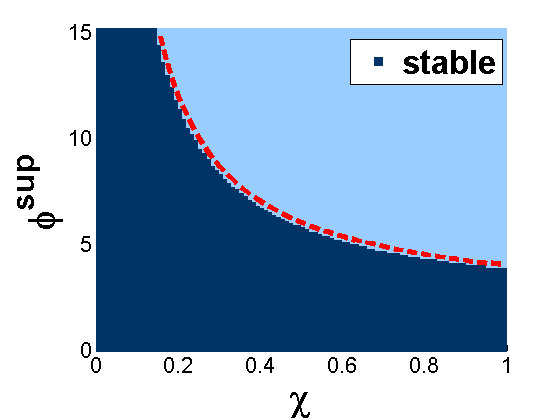
\includegraphics[width=\textwidth]{./fig/param2.png}
		\caption{Parameter space.}
		\label{fig:paramSpace}
	\end{subfigure}  
	%\\
	\begin{subfigure}[t]{0.55\linewidth}
		\centering
		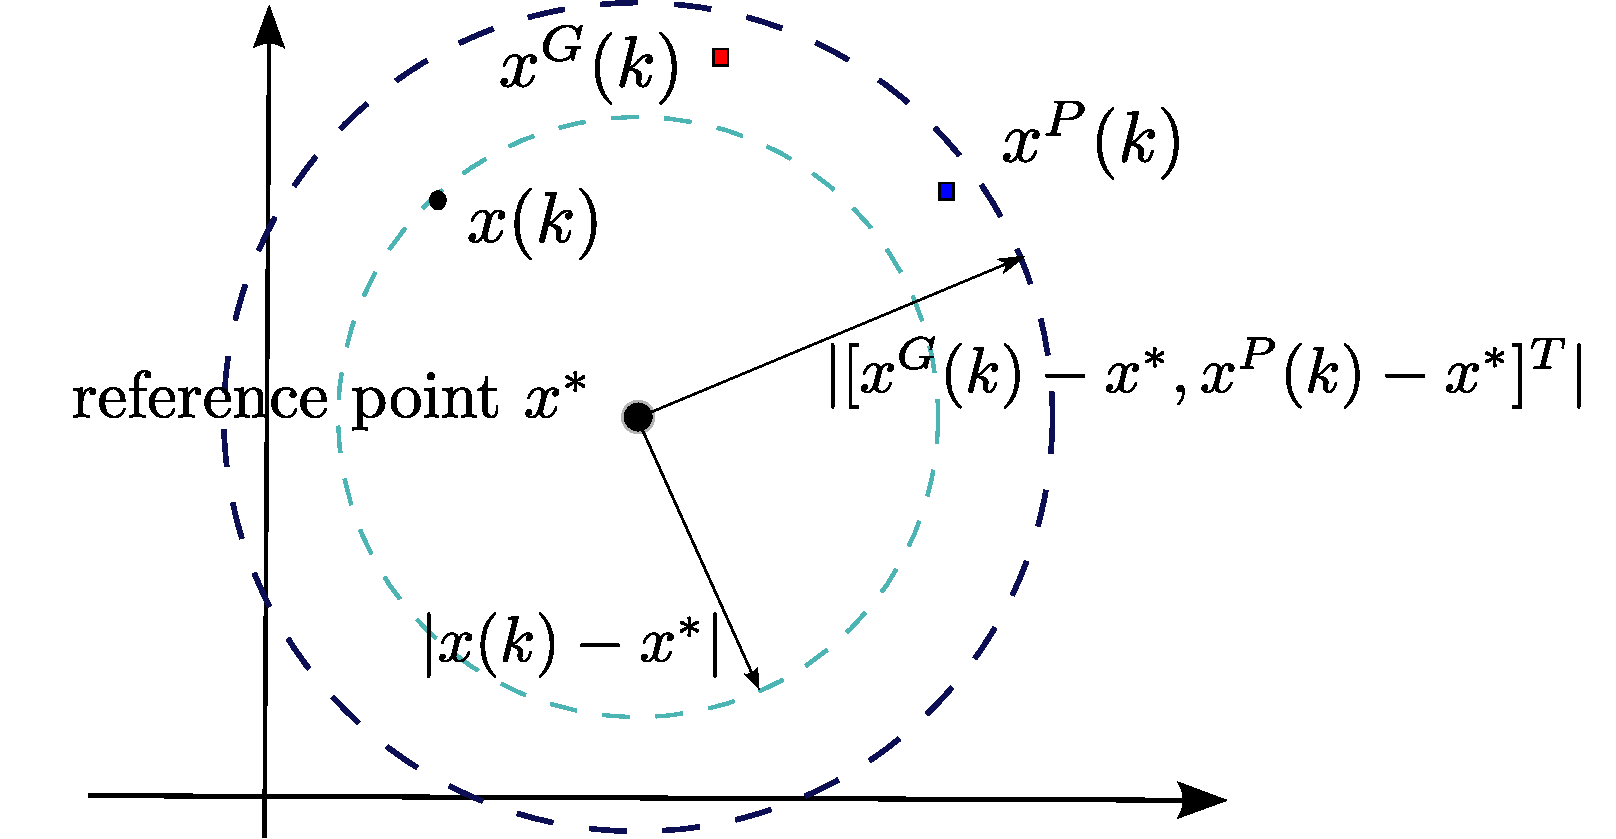
\includegraphics[width=\textwidth]{./fig/boundary}
		\caption{A bound on a particle's position by a reference point $ x^{*} $ from Equation %\eqref{eq:state_bound:conv}.
		The ratio of two radii indicates $ \gamma $..}
		\label{fig:boundary}
	\end{subfigure}   
	\caption{Parameter space and the boundary of a particle.}
	\label{fig:particle:param_bound}
\end{figure}

Given an input-to-state stable position-update component, we will see that the convergence of $ x_{i}(k) $ depends on bounds on $ x^{G}_{i}(k) $ and $ x^{P}_{i}(k) $.
Figure \ref{fig:boundary} illustrates a boundary on the particle motion, which indicates the exploring capability and exploitation property of one particle.
As in the Figure \ref{fig:sys:swarm}, the particles in the swarm form a networked feedback structure.
Integrating the input-to-state stability of each component in the swarm helps us understand the convergence of the swarm.
This helps us to analyze the capability of optimal search of the PSO in different fitness landscapes with different parameter selections.


%%%%%%%%%%%%%%%%%%%%%%%%%%%%%%%%%%%%%%%%%%%%%%%%%%%%%%%%%%%%%%%%%%%%%%%%%%%%%%%
% Change these to reflect the bibliography style and bibtex database file you want to use
\bibliographystyle{plain}
\bibliography{proposal_ref}

\end{document}
